\documentclass{simcenterdocumentation}
%% \usepackage[letterpaper, margin=1in]{geometry}

\usepackage{epsf}
%\usepackage{times}
\usepackage{latexsym}
\usepackage{amsbsy}
\usepackage{ifthen}

%\usepackage[sort&compress,square,comma,authoryear]{natbib}
%\usepackage[round]{natbib}
\usepackage{color, soul}
\usepackage{fancyhdr}	% Package to create Headers and Footers
\usepackage{tabu, tabulary, tabularx} 	% packages for tables
\usepackage{multirow}
\usepackage{float}
\usepackage{booktabs}
\usepackage{enumerate, enumitem}
\usepackage{graphicx}
\usepackage[hypcap,justification=centerlast,labelfont=bf,font=small]{caption}
\usepackage{pdflscape}
\usepackage{xfrac}
\usepackage{arydshln}
%\usepackage[sc]{titlesec}
\usepackage{subcaption}
\usepackage{hyperref}
\usepackage{amsmath,amssymb,mathrsfs}
\usepackage{epstopdf}
%\usepackage[tight,footnotesize]{subfigure}
\usepackage{dcolumn}
\usepackage{bm}
\usepackage[super]{nth}
\usepackage{todonotes}
\usepackage{pdfpages}
\usepackage[numbers,sort]{natbib}
\usepackage[capitalize,nameinlink,noabbrev]{cleveref}
%\usepackage[round]{natbib}   % omit 'round' option if you prefer square brackets
%\bibliographystyle{plainnat}
\usepackage{hyperref}
\hypersetup{
  colorlinks   = true,    % Colors links instead of ugly boxes
  urlcolor     = blue,    % Color for external hyperlinks
  linkcolor    = blue,    % Color of internal links
  citecolor    = blue      % Color of citations
}





% Commands %%%%%
	\newcommand{\mb}[1]{$\mathbf{#1}$}
	%% \newcommand{\bs}[1]{\boldsymbol #1}
	\newcommand{\intwo}{\ensuremath{\,\mathrm{in}^2}}
	\newcommand{\ksi}{\ensuremath{\,\mathrm{ksi}}}
	\newcommand{\kip}{\ensuremath{\,\mathrm{k}}}
	\newcommand{\psf}{\ensuremath{\,\mathrm{psf}}}
	\newcommand{\kips}{\ensuremath{\,\mathrm{kips}}}
	\newcommand{\ftk}{\ensuremath{\,\mathrm{ft-k}}}
	\newcommand{\ink}{\ensuremath{\,\mathrm{in-k}}}
	\newcommand{\ft}{\ensuremath{\,\mathrm{ft}}}
	\newcommand{\m}{\ensuremath{\,\mathrm{m}}}
	\newcommand{\inch}{\ensuremath{\,\mathrm{in}}}
	\newcommand{\pdiff}[2]{\frac{\partial#1}{\partial#2}}
	\newcommand{\solution}[1]{\color{blue!40!black}{\fbox{\begin{minipage}{0.933\textwidth}
								{#1}\end{minipage}}}\color{black}}
	
	\newcommand{\atena}{ATENA}

%%%%%%%% TITLE %%%%%%%%
\DeclareFixedFont{\bigsf}{OT1}{cmr}{b}{sc}{25}%{T1}{cmr}{b}{sc}{0.5in}
%\title{\bigsf{Investigation of Stiffness Irregularity in RC Walls}}
%% \title{\bigsf{EVW Tool Examples}}
%% \date{}
%\author{Kamal A. Ahmed}






%%%%%%%%%%%%%%%%%%%%%%%%%%%%%%%%%%%%%%%%%%%%%%%%%%%%%%%%%%%%%%%%%%%%%%%%%%%%%%%%%%
%					Beginning the document										 %
%%%%%%%%%%%%%%%%%%%%%%%%%%%%%%%%%%%%%%%%%%%%%%%%%%%%%%%%%%%%%%%%%%%%%%%%%%%%%%%%%%

\begin{document}
\title{Earthquake versus Wind (EVW) Application Study Questions}

% Use superscripts to indicate author affiliations
\author{Kamal A. Ahmed \& Laura Lowes}
%\author{Moe Howard$^{1,2}$ Larry Fine$^1$ Curly Howard$^2$}
\institutions{NHERI SimCenter, University of Washington}
\softwarename{EVW}
\softwareversion{1.0.0}
\softwarepage{https://simcenter.designsafe-ci.org/learning-tools/evw-application/}

\hypersetup{pageanchor=false}
\maketitle
\copyrightpage
\acknowledgments


%\maketitle
%\addcontentsline{toc}{section}{Front Page}
%
%\newpage
%\tableofcontents
%\addcontentsline{toc}{section}{Contents}

\graphicspath{{figures/}{}}

\renewcommand{\thesection}{Problem \arabic{section}}
\renewcommand{\thesubsubsection}{Problem \arabic{subsubsection}}
\section*{Study Questions}

\subsubsection{\label{sec:p1}Drift, velocity and acceleration (walled building)} Use the \getsoftwarepage{\texttt{\getsoftwarename{}} app} to analyze the 12-story walled building shown in \cref{fig:plan}. The building has a damping ratio of 2\%. Story stiffness is 5000.0 k/in. For wind, assume an exposure category $B$ and a gust wind speed of 95.0 mph. Total building weight is 30000.0 kips and is equal for all floors including the roof. Also $F_y = 60 \ksi$ and hardening ratio, $b = 0.02$. Analyze the building using both PDelta enabled and disabled. Explore the followings:
\begin{enumerate}[label=\alph*)]
	\item Maximum roof drifts under wind and earthquake loading
	\item Maximum first story and $12^\mathrm{th}$ story drifts
          for the two load cases. How do these compare with the
          maximum roof drift?
	\item Maximum story velocity
	\item Maximum story acceleration
	\item Why are story drift, verlocity and acceleration
          important quantities to consider?
\end{enumerate}

\begin{figure}[H]
	\centering 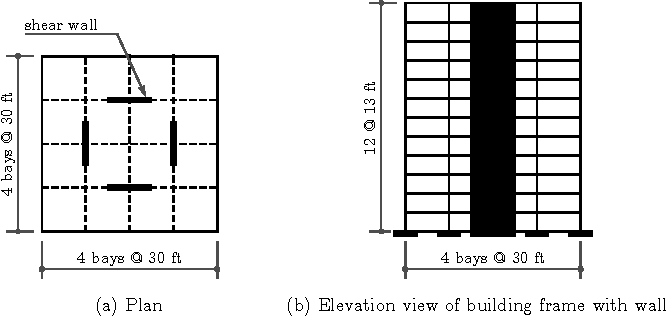
\includegraphics[scale=1]{plan.pdf}
	\caption{Geometries of the 12-story building.}
	\label{fig:plan}
\end{figure} 


\subsubsection{Effect of damping ratio (walled building)} Analyze the building of \ref{sec:p1} (\cref{fig:plan}) again but this time use a damping ratio of 5\% and compare the results of the two problems and explain the differences. Which building is safer when exposed to the same earthquake excitation? What causes building damping? What might cause increased damping?

\subsubsection{Effect of hardening ratio (walled building)} What happens if you analyze the building shown in \cref{fig:plan} with no hardering ratio ($b = 0$)? And what will change if hardening ratio is increased to $b = 0.05$? What properties determine the story hardening ratio?


\subsubsection{Drift, velocity and acceleration (moment-resisting frame)} Considering \textsl{East-West} direction, for the moment-frame building shown in \cref{fig:5story_steel_frame} calculate the stiffness of the each story. For stiffness calculations only take the moment resisting frames into cosideration. Beam and column sections are given in \cref{tab:tab1}. Columns in the moment resisting frame are bending about their strong axes.

Assume 2\% damping for the building and exposure category $B$ with a gust wind speed of 110.0 mph. Loading is as follows:
\begin{table}[H]
\centering
\begin{tabular}{ccc}
Story			& Dead load	(psf)		& Live load	(psf)	\\ \cmidrule(rl){1-1}\cmidrule(rl){2-2}\cmidrule(rl){3-3}
Floors			& 100				& 20			\\
Roof			& 80				& 15			
\end{tabular}
\end{table}
While $F_y = 50 \ksi$ and $b = 0$, analyze the building for both earthquake and wind using \getsoftwarepage{\texttt{\getsoftwarename{}} app}. Do not consider $P-\Delta$ effect. Explore the followings:

\begin{enumerate}[label=\alph*)]
	\item Maximum roof drifts under wind and earthquake loading
	\item Maximum first story and $5^\mathrm{th}$ story drifts for the two load cases. How do these compare with the maximum roof drift?
	\item Maximum story velocity
	\item Maximum story acceleration
	\item Why are story drift, verlocity and acceleration important quantities to consider?
\end{enumerate}

\begin{figure}[H]
	\centering 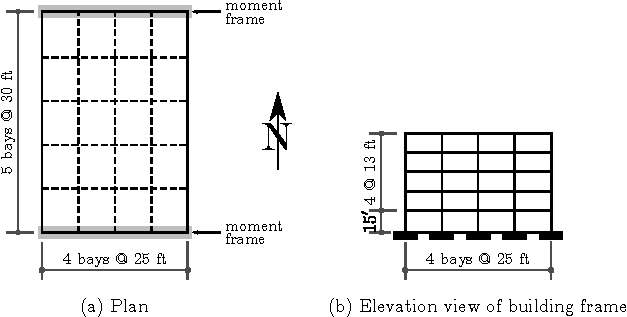
\includegraphics[scale=1]{5story_steel_frame.pdf}
	\caption{Elevation and plan of the 5-story steel moment-frame building.}
	\label{fig:5story_steel_frame}
\end{figure}
\begin{table}[H]
	\centering \caption{Beams and columns of the moment resisting frame.}
	\label{tab:tab1}
	\begin{tabular}{ccc} \toprule
	Story/Floor			& Columns						& Beams
	\\ \midrule
	1/2					& $\mathrm{W14 \times 311}$		& $\mathrm{W30 \times 116}$	\\
	2/3					& $\mathrm{W14 \times 311}$		& $\mathrm{W30 \times 116}$	\\
	3/4					& $\mathrm{W14 \times 311}$		& $\mathrm{W30 \times 116}$	\\
	4/5					& $\mathrm{W14 \times 311}$		& $\mathrm{W30 \times 116}$	\\
	5/Roof				& $\mathrm{W14 \times 257}$		& $\mathrm{W24 \times 62}$	\\ \bottomrule
	\end{tabular}
\end{table}


\subsubsection{Effect of damping ratio (moment-resisting frame)} Redo the analysis of the building shown in \cref{fig:5story_steel_frame} for a damping ratio of 5\% and compare the results of the two problems and explain the differences. What differences do you observe and why? What causes building damping? What might cause increased damping?

\subsubsection{Effect of hardening ratio (moment-resisting frame)} Redo the analysis of the building shown in \cref{fig:5story_steel_frame} but use $b = 0.05$ and keep the damping ratio as 2\%. Is there any changes? If yes, why and what is the effect of these differences on the overall behavior of the building?  What properties determine the story hardening ratio?

\subsubsection{$P-\Delta$ effects (moment-resisting frame)} Re-analyze the building shown in \cref{fig:5story_steel_frame} but this time account for $P-\Delta$ effects. Comment on the differences.

\subsubsection{Stiffer building (walled building)} Re-analyze the building shown in \cref{fig:plan} but increase the stiffness by 25\%. What observations can you make?

\subsubsection{Stiffer building (moment-resisting frame)} Re-analyze the building shown in \cref{fig:5story_steel_frame} and increase the stiffness by 25\%. What observations can you make?

\subsubsection{Soft story (Walled building)} An architect decides to insert a door opening in the lateral resisting element (shear walls) of the building shown in \cref{fig:plan}. The openings are only in the first story and reduce the story stiffness by 50\%. Re-analyze this building, taking into account the opening in the shear wall, and compare the results with the original case. Comment on the results and observations you make.



\end{document}
